\chapter{Experimentos}
\label{cap:capitulo7}

\begin{flushright}
\begin{minipage}[]{10cm}
\emph{Toda la vida es un experimento. Cuantos más experimentos hagas, mejor.}\\
\end{minipage}\\

Ralph Waldo Emerson\\
\end{flushright}

\vspace{1cm}

\setcounter{footnote}{117} % Establecer la numeración de la siguiente nota al pie

En este capítulo se tratarán los diferentes experimentos llevados a cabo para la realización de este proyecto y que han permitido conseguir y demostrar la consecución del objetivo y subobjetivos definidos en la Sección \ref{sec:descripcion}.

\section{Impresión 3D}
\label{sec:expimpresion3d}
Aparte de la solución proporcionada en la Sección \ref{sec:impresionmontaje}, se probaron previamente distintas opciones de diseño y de impresión 3D hasta encontrar la mejor opción.

Primero, se optó por diseñar la estructura como una pieza única para facilitar el trabajo de ensamblaje para los usuarios, sin embargo el resultado final no fue el esperado (Figura \ref{fig:imfallida}). 

\begin{figure}[ht!]
	\centering
	\begin{minipage}{0.45\linewidth}
		\centering
		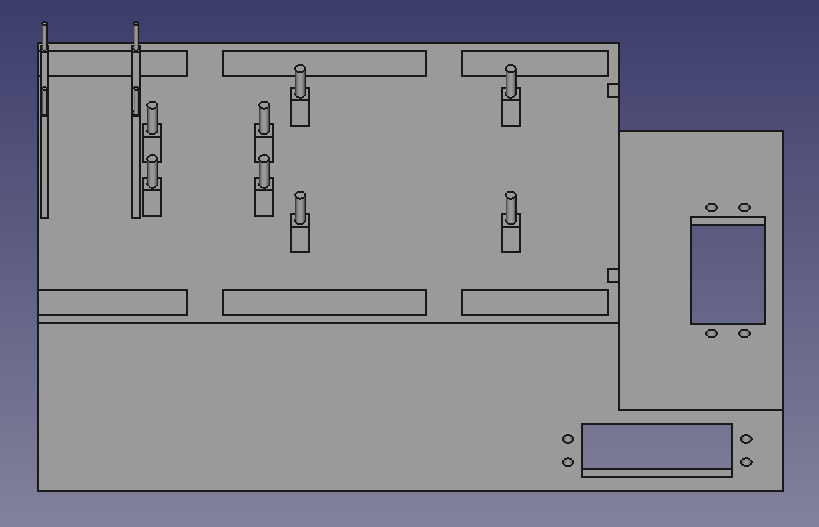
\includegraphics[width=\linewidth]{figs/cap7/impresionfallida1.png}
	\end{minipage}
	\hspace{1cm}
	\begin{minipage}{0.40\linewidth}
		\centering
		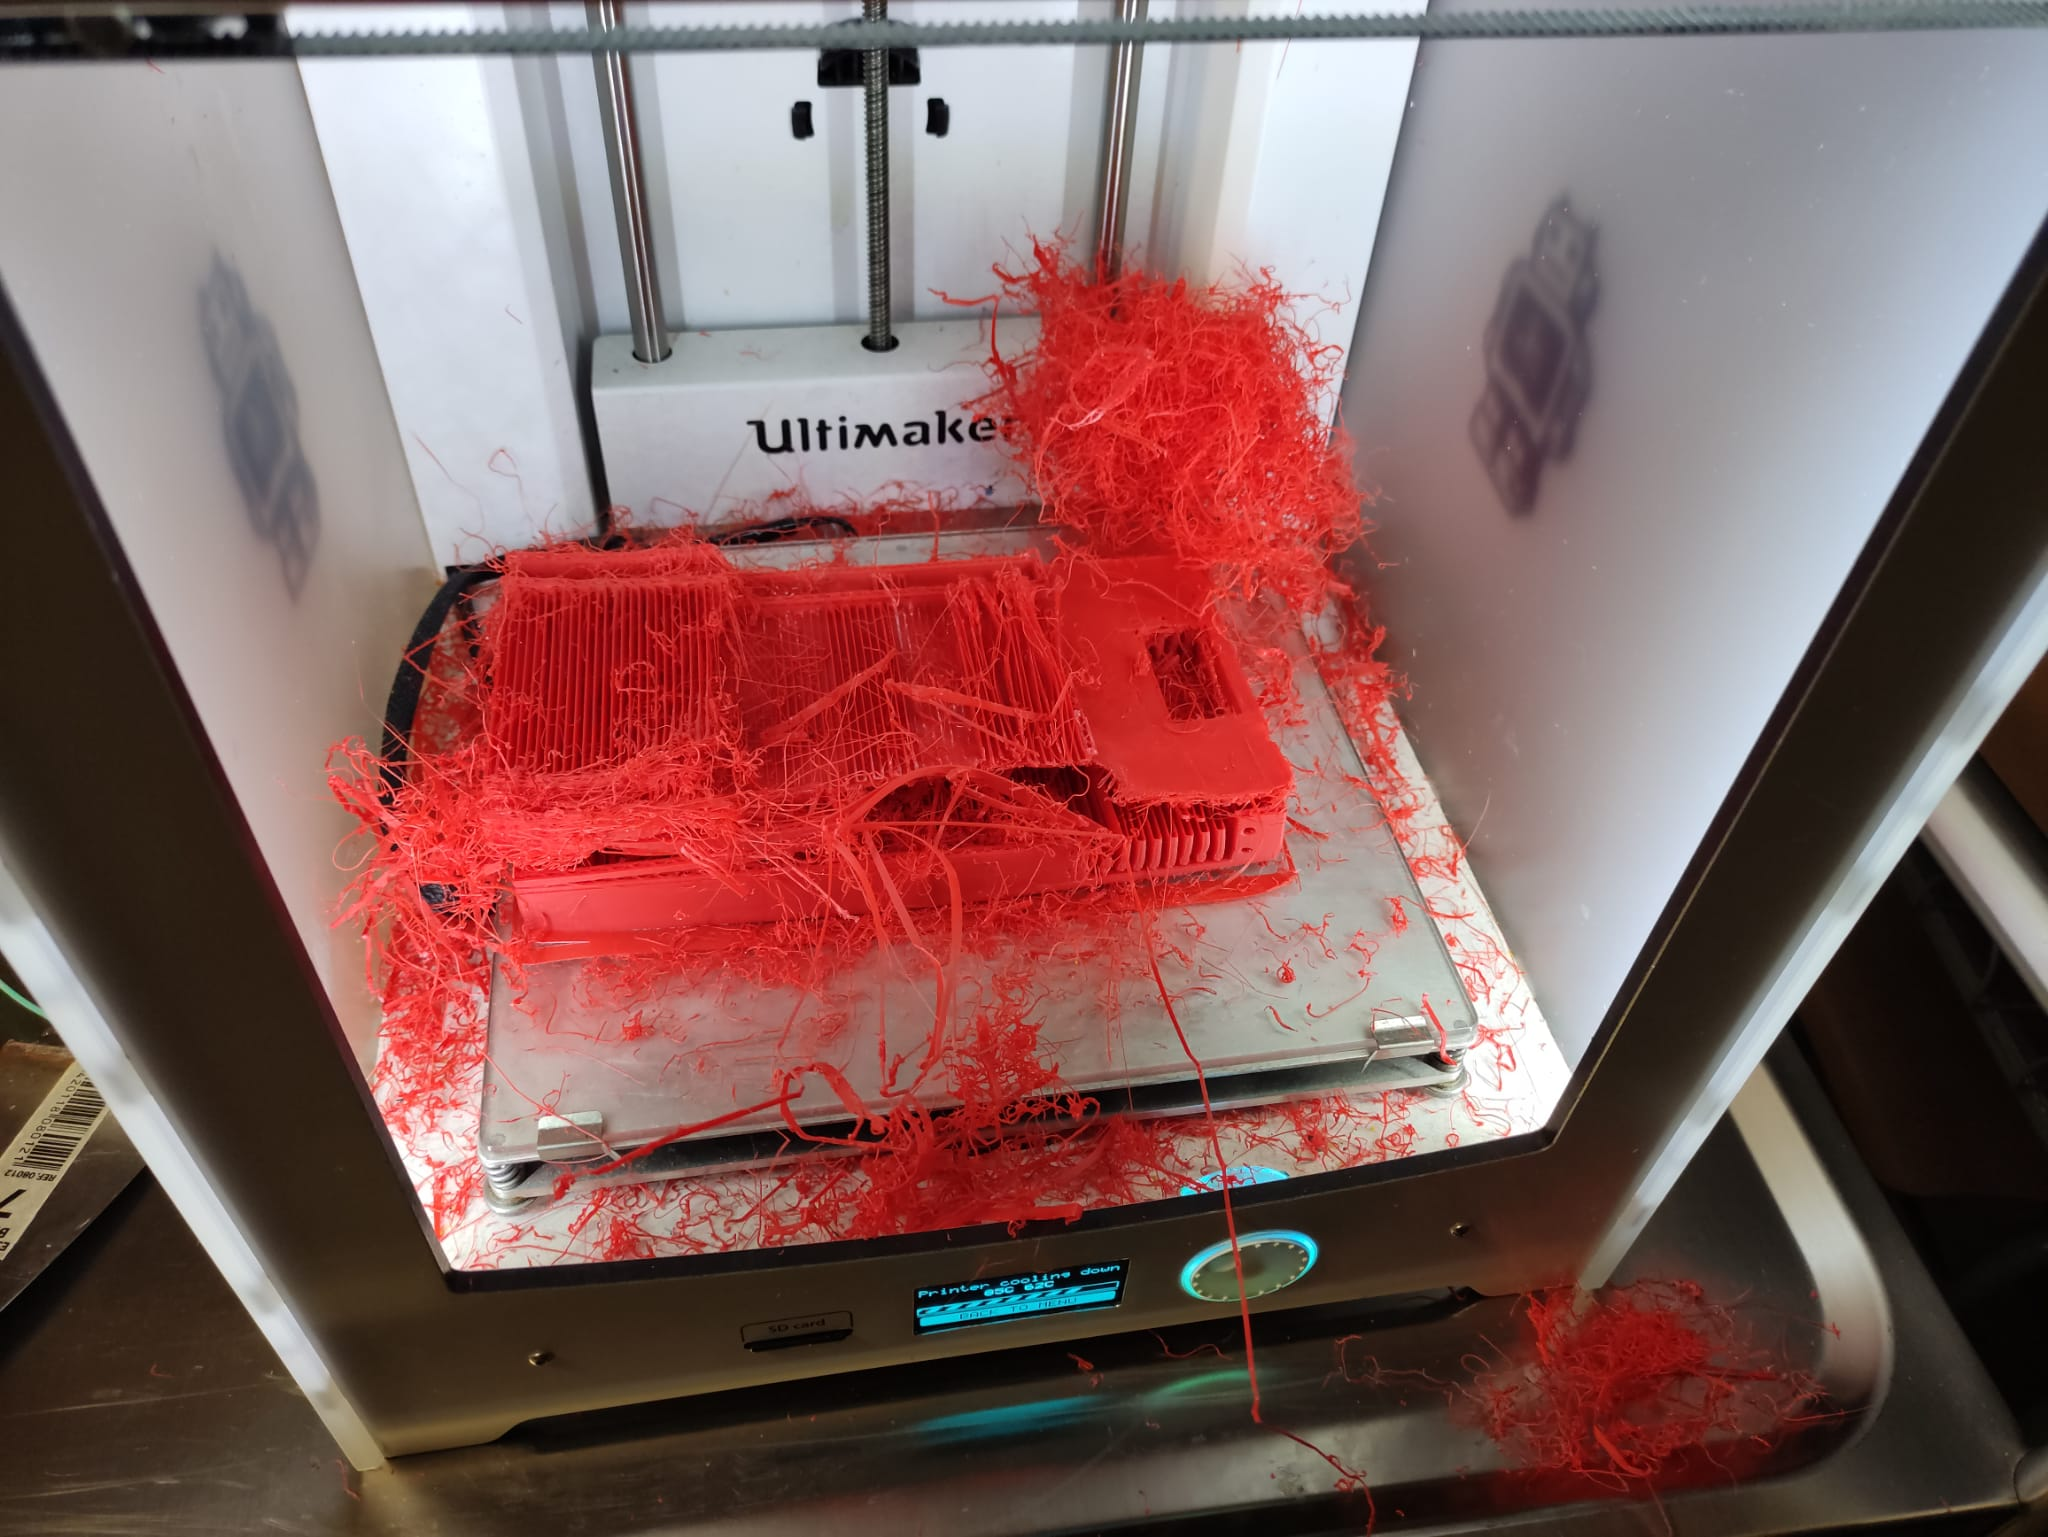
\includegraphics[width=\linewidth]{figs/cap7/piezav1error.jpeg}
	\end{minipage}
	\caption{Versiones previas de impresión}
	\label{fig:imfallida}
\end{figure}

Después de eso, se tuvo que cambiar el enfoque y se decidió dividirlo en diferentes piezas para intentar solucionar el problema, como se comentó en la Sección \ref{sec:diseñocad}. En ese momento se estaba usando otra impresora distinta a la definida en la Sección \ref{sec:impresionmontaje}, llamada Ultimaker Cura 2+\footnote{\url{https://ultimaker.com/3d-printers/s-series/ultimaker-2-connect/}}y se empleó ABS en vez de PLA; por lo tanto, los parámetros de impresión fueron distintos (Cuadro \ref{cuadro:cimpresion2}), pero se producía \textit{warping}. Para conocer más acerca de distintas pruebas, puedes consultarlas en la Wiki\footnote{\url{https://github.com/RoboticsURJC/tfg-jlopez/wiki/HARDWARE\#impresi\%C3\%B3n-3d}}.

\begin{table}[H]
	\begin{center}
		\begin{tabular}{|c|c|}
			\hline
			Características & Parámetros\\
			\hline
			 Densidad & 1.04 g/cm³\\
			\hline
			Diámetro & 2.85 mm\\
			\hline
			Temperatura de impresión & 240 ºC\\
			\hline
			Temperatura de la placa & 110 ºC\\
			\hline
			Temperatura en modo de espera & 175 ºC\\
			\hline
			Distancia de retracción & 6.50 mm\\
			\hline
			Velocidad de retracción & 40mm/s\\
			\hline
			Velocidad del ventilador & 10\%\\
			\hline
		\end{tabular}
		\caption{Características usadas en impresiones previas}
		\label{cuadro:cimpresion2}
	\end{center}
\end{table}

\section{Ruedas}
\label{sec:expruedas}
Como se comentó en la Sección \ref{subsec:ruedas}, en este proyecto se han usado dos tipos de ruedas que gracias a las distintas pruebas realizadas, se ha podido definir las características de cada una de ellas. 

En el primer vídeo\footnote{\url{https://www.youtube.com/watch?v=G71mNFDIDuw}} (Figura \ref{fig:pruebaruedas} izquierda) se puede ver a PiBotJ usando las ruedas finas negras y teniendo dificultades en superficies con irregularidades. Por otro lado, en el segundo vídeo\footnote{\url{https://www.youtube.com/watch?v=BYluIeGEo6Q}} (Figura \ref{fig:pruebaruedas} derecha) se puede ver a PiBotJ usando las ruedas azules genéricas, más anchas, y superando con mayor facilidad las dificultades que con las ruedas del kit \textit{ActivityBot}.

%% Incluir 2 vídeos y las dos fotos (capturas del video)

\begin{figure}[ht!]
	\centering
	\begin{minipage}{0.45\linewidth}
		\centering
		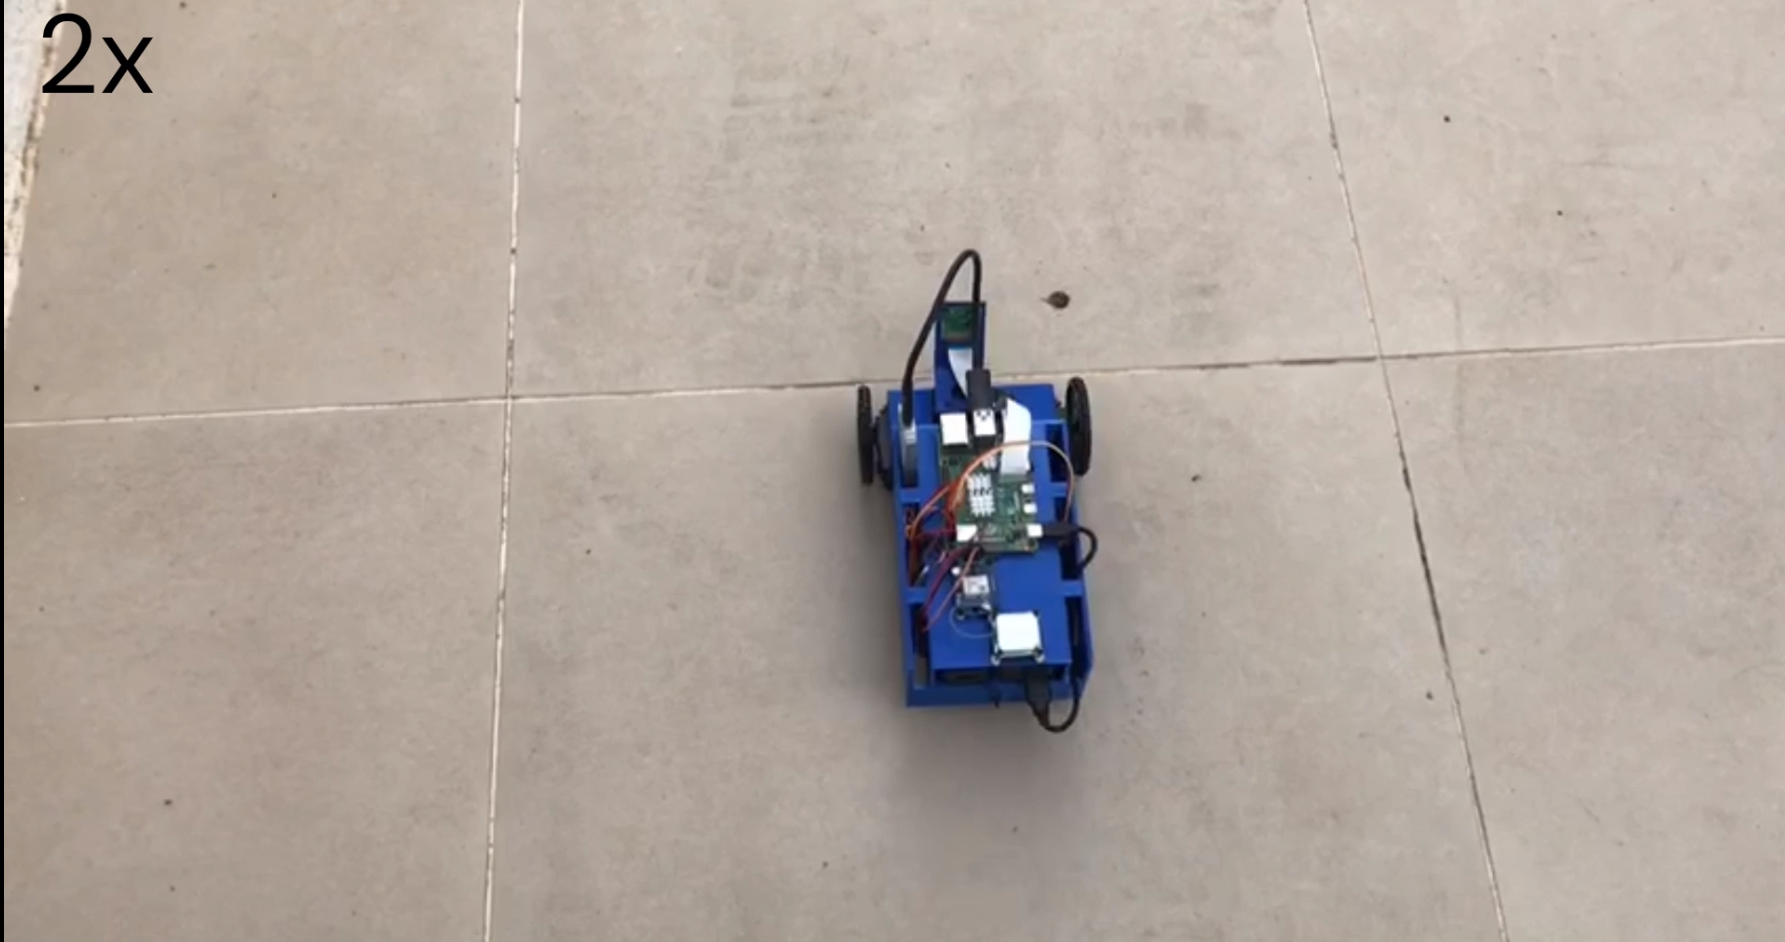
\includegraphics[width=\linewidth]{figs/cap7/pruebanegra.png}
	\end{minipage}
	\hspace{1cm}
	\begin{minipage}{0.45\linewidth}
		\centering
		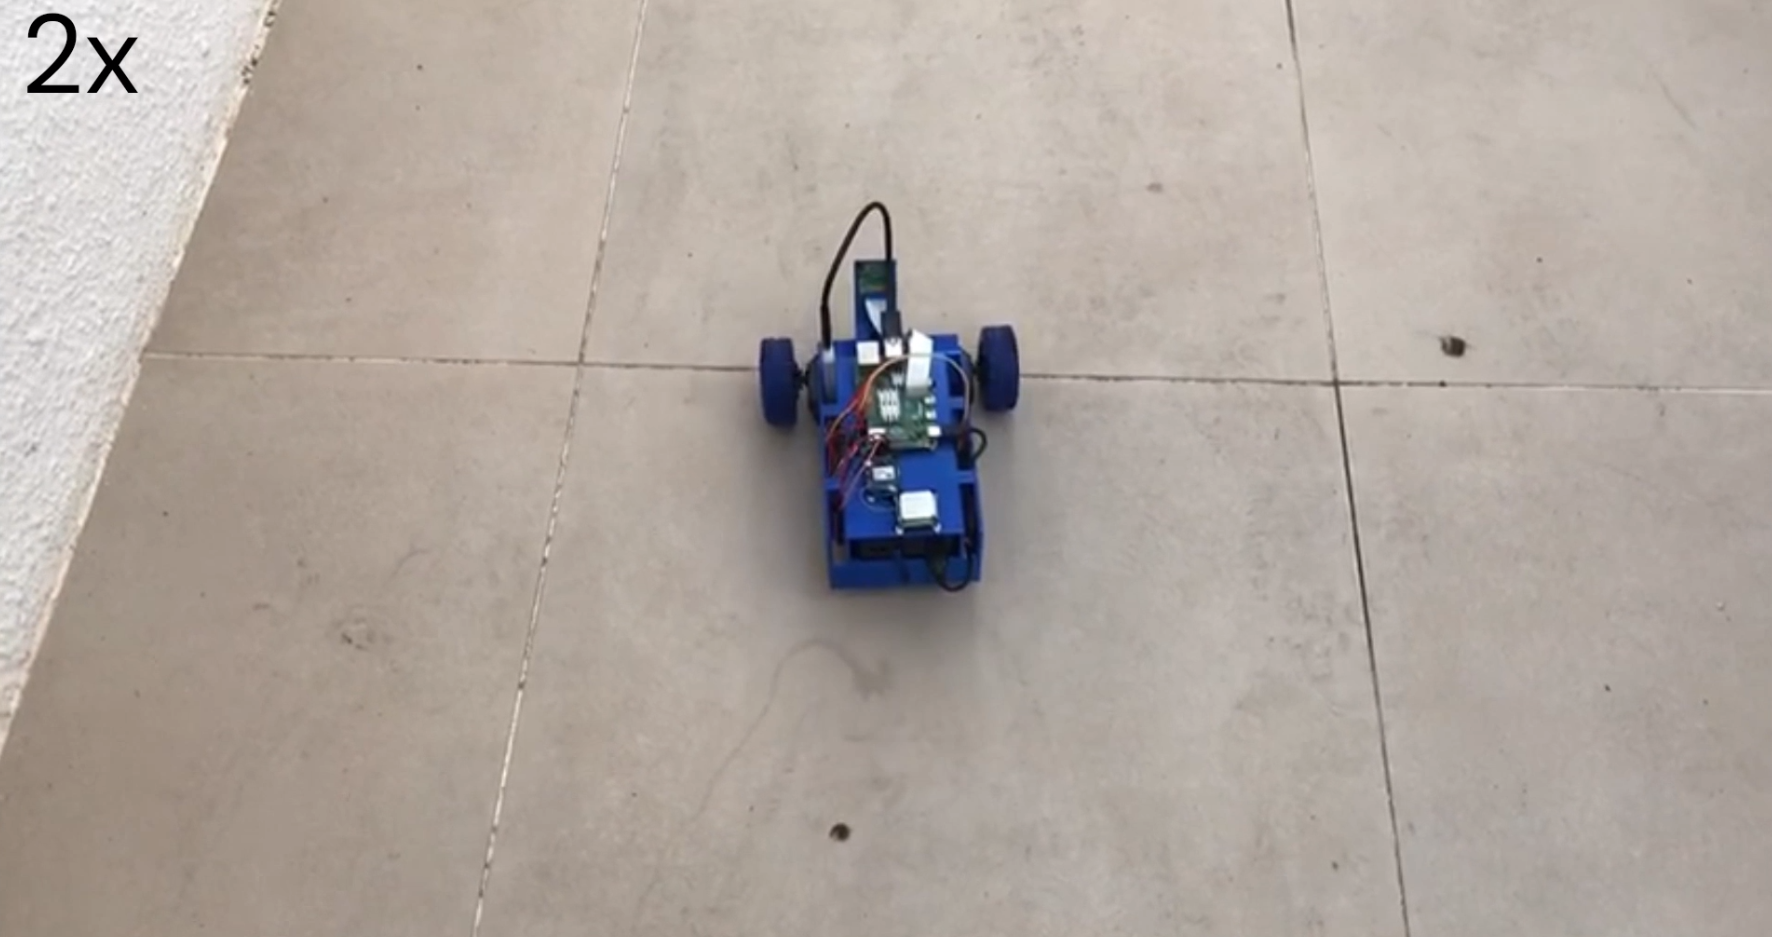
\includegraphics[width=\linewidth]{figs/cap7/pruebaazul.png}
	\end{minipage}
	\caption{Capturas de las pruebas de PiBotJ con las distintas ruedas}
	\label{fig:pruebaruedas}
\end{figure}


\section{Detección de baches}
\label{sec:expaa}

%Para conseguir el modelo de entrenamiento de red neuronal creado con YOLOv8, con formato .pb, que se explicó en la Sección \ref{subsec:softwareiayolo}, se realizaron numerosas pruebas, pero finalmente para la etapa de entrenamiento se decidió usar la siguiente configuración (Figura \ref{fig:configaa}). Está completamente recogido y facilitado en el fichero \verb|args.yaml|\footnote{\url{https://github.com/RoboticsURJC/tfg-jlopez/blob/main/code/ros2/src/pibotj_rr/custom_model_lite/args.yaml}}.

%\begin{figure} [h!]
%	\begin{center}
%		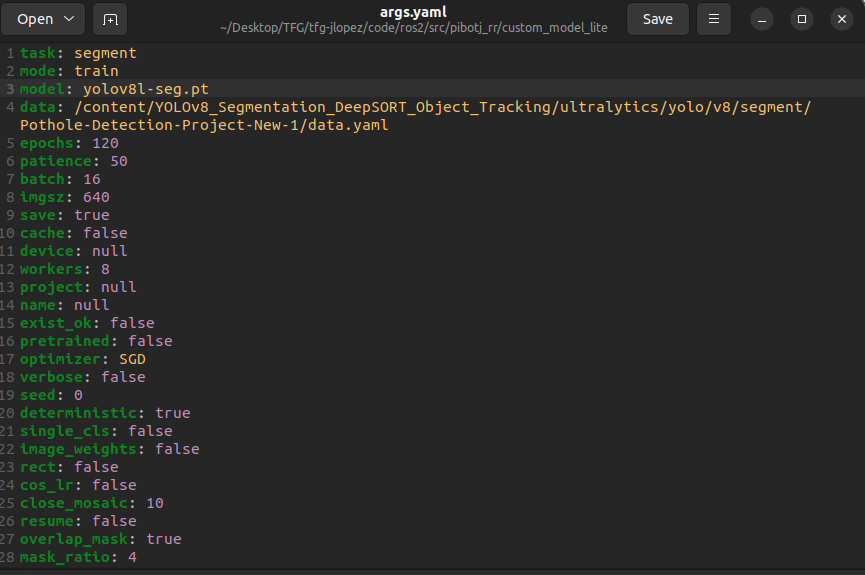
\includegraphics[width=12cm]{figs/cap7/args.png}
%	\end{center}
%	\caption{Parte de la configuración usada para el entrenamiento}
%	\label{fig:configaa}
%\end{figure}

%% Descripción de la imagen 

Una vez creado, entrenado y convertido el modelo en el formato .tflite, formato compatible con Google Coral, se crearon distintas versiones que se describen a continuación.  
\begin{itemize}
	\item \verb|detect.tflite|\footnote{\url{https://github.com/RoboticsURJC/tfg-jlopez/blob/main/code/ros2/src/pibotj_rr/custom_model_lite/detect.tflite}}. Esta primera versión se realizó usando un dataset de 75 imágenes pero usa CPU y tiene baja reactividad: tiene una latencia de unos cuatro segundos.
	\item \verb|detect_edgetpu.tflite|\footnote{\url{https://github.com/RoboticsURJC/tfg-jlopez/blob/main/code/ros2/src/pibotj_rr/custom_model_lite/detect_edgetpu.tflite}}. Esta versión usa el dataset de 75 imágenes y se intentó que el modelo usase \ac{TPU} del Google Coral pero no funcionó.
	\item \verb|best_full_integer_quant_edgetpu.tflite|\footnote{\url{https://github.com/RoboticsURJC/tfg-jlopez/blob/main/code/ros2/src/pibotj_rr/custom_model_lite/best_full_integer_quant_edgetpu.tflite}}. Esta versión usa el dataset definido en la Sección \ref{subsec:softwareiayolo}. En esta ocasión sí es capar de usar \acs{TPU} pero el modelo se moría a los pocos segundos de inicializarlo y era debido a que procesaba imágenes demasiado grandes.
	\item \verb|bestv2_full_integer_quant_edgetpu.tflite|\footnote{\url{https://github.com/RoboticsURJC/tfg-jlopez/blob/main/code/ros2/src/pibotj_rr/custom_model_lite/bestv2_full_integer_quant_edgetpu.tflite}}. Esta es la la versión actual usada en el proyecto. A diferencia del ejemplo anterior, esta versión procesa imágenes de 192x192 y así evitamos que el modelo se muera y funcione perfectamente. La latencia se ha reducido a más de un cuarto de la primera versión y permite el correcto funcionamiento del modelo.	
\end{itemize}


En la Sección \ref{subsec:softwareiayolo} también se comenta cómo conseguir que los valores obtenidos sean estables usando \acs{EMA} y a continuación se puede ver dos gráficas que demuestra la aplicación EMA sobre la máscara de la clase 0 y la máscara de la clase 1 (Figura \ref{fig:diagramaemac0} y Figura \ref{fig:diagramaemac1} respectivamente).

%\begin{figure} [h!]
%	\begin{center}
%			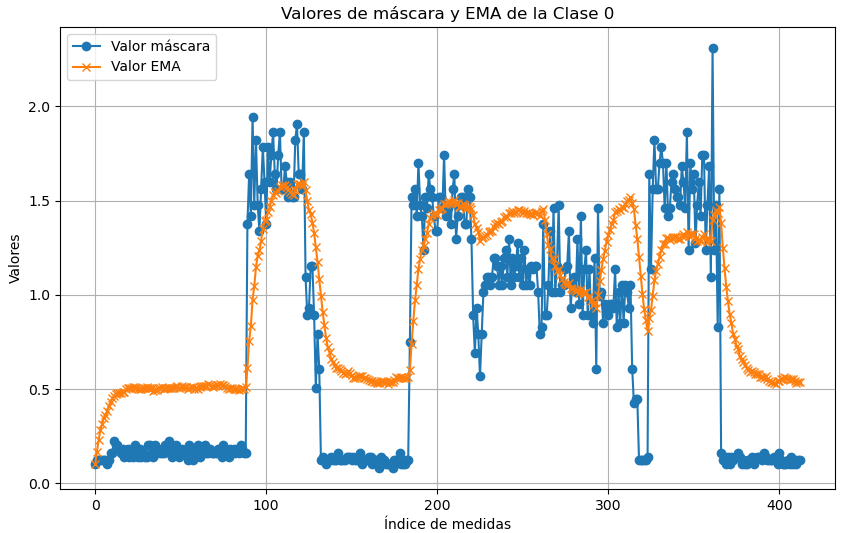
\includegraphics[width=15cm]{figs/cap7/GraficaC0.png}
%		\end{center}
%	\caption{Gráfica que muestra los valores de la clase 0}
%	\label{fig:diagramaemac0}
%\end{figure}

En Figura \ref{fig:diagramaemac0}\footnote{Los valores usados en la gráfica se pueden apreciar aquí: \url{https://github.com/RoboticsURJC/tfg-jlopez/blob/main/code/ros2/ema_experiments/valoresc0.csv}}, se puede ver que los valores por encima de 0.6 es cuando se detecta que hay bache. Los valores azules en todo momento se puede ver cómo toman valores dispares, mientras que los valores naranjas permiten que el valor se estabilice eliminando picos. Si se produce un pequeño movimiento y se pierde momentáneamente el bache, gracias a EMA tarda muy poco en recuperar el valor previo, como ocurre en el intervalo entre las medidas 200 y 300.

\begin{figure} [h!]
	\begin{center}
		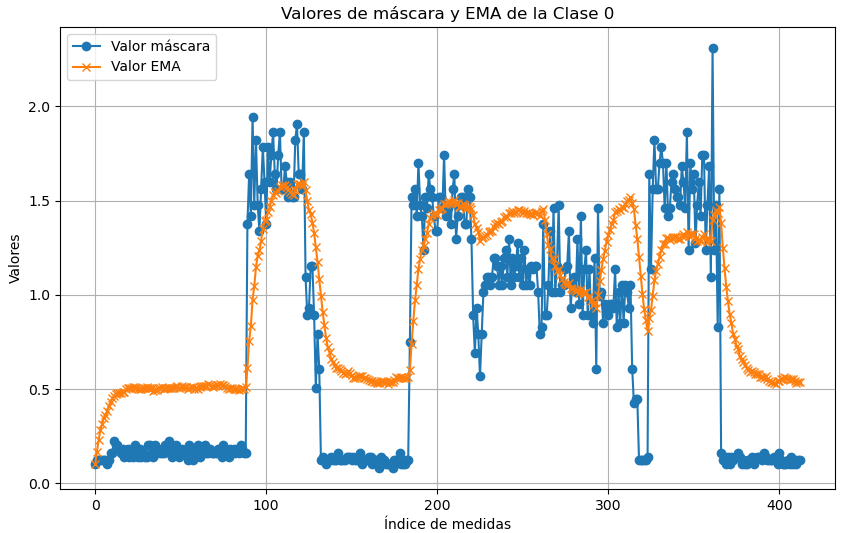
\includegraphics[width=11.5cm]{figs/cap7/GraficaC0.png}
	\end{center}
	\caption{Gráfica que muestra los valores de la clase 0}
	\label{fig:diagramaemac0}
\end{figure}

%\begin{figure} [h!]
%	\begin{center}
%		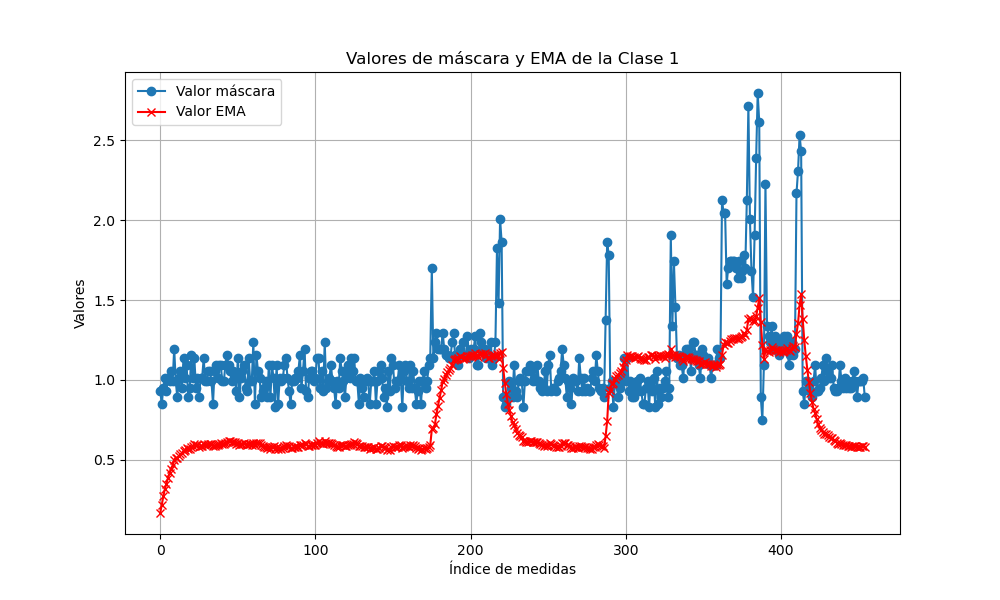
\includegraphics[width=15cm]{figs/cap7/GraficaC1.png}
%	\end{center}
%	\caption{Gráfica que muestra los valores de la clase 1}
%	\label{fig:diagramaemac1}
%\end{figure}

Sin embargo, en la Figura \ref{fig:diagramaemac1}\footnote{Los valores usados en la gráfica se pueden apreciar aquí: \url{https://github.com/RoboticsURJC/tfg-jlopez/blob/main/code/ros2/ema_experiments/valoresc1.csv}} se puede apreciar cómo inicialmente los valores azules que no muestran bache están por encima del umbral elegido y es gracias a EMA que los valores se estabilizan por debajo del umbral, teniendo a lo largo de todo el proceso un comportamiento correcto. 

\begin{figure} [h!]
	\begin{center}
		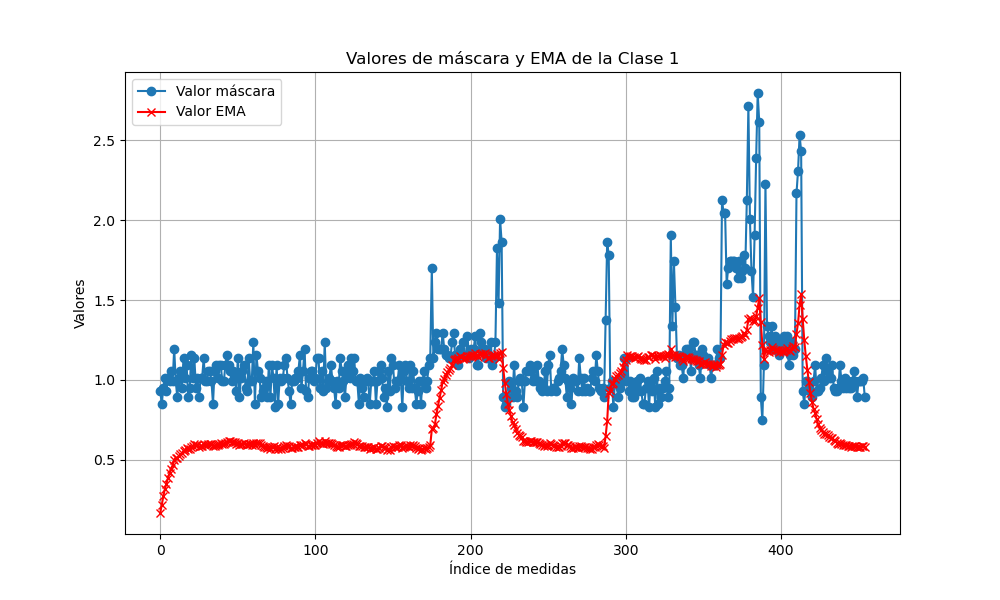
\includegraphics[width=11.5cm]{figs/cap7/GraficaC1.png}
	\end{center}
	\caption{Gráfica que muestra los valores de la clase 1}
	\label{fig:diagramaemac1}
\end{figure}

\subsection{Obtención del contorno y coordenadas del bache}
\label{subsec:expcontorno}

Para la obtención de las coordenadas del bache detectado, se probaron distintas opciones. La primera de ellas fue tomar la imagen en la que se consideraba que tenía bache y, a partir de ella, aplicando un desenfoque gaussiano, convirtiéndola en escala de grises, se aplicó el detector de bordes de Canny, utilizando a ojo 80 como umbral mínimo y 180 como umbral máximo. El problema que tenía esta opción era que el contorno a buscar se aplicaba a toda la imagen y no solo dónde se encontraba el bache, produciéndose en ocasiones la detección incorrecta (Figura \ref{fig:contornoerror}).

\begin{figure} [h!]
	\begin{center}
			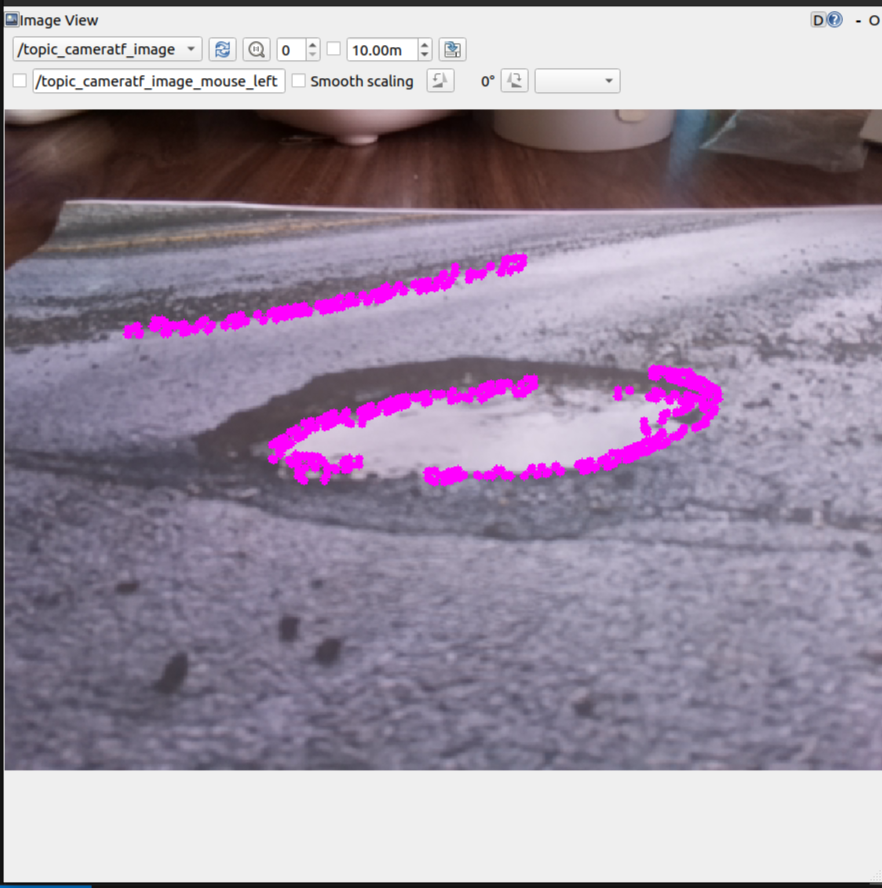
\includegraphics[width=6cm]{figs/cap7/contornoerror.png}
		\end{center}
	\caption{Primera versión en la obtención del contorno del bache}
	\label{fig:contornoerror}
\end{figure}

La segunda y última opción para realizar la detección del contorno, descrita en la Sección \ref{subsec:softwareiayolo} y se puede ver gracias al Código \ref{cod:contorno}. Siendo el valor de 0,6 en el paso de binarizar la máscara, el elegido para decidir si hay bache o no en la imagen. El resultado final se muestra en la Figura \ref{fig:contornobache}.

\begin{code}[h]
	\begin{lstlisting}[language=Python]
		def extract_contour_pixels(self, pothole_mask, resized_frame):
			# Escalar para que aparezca en el tamano correcto
			scale_factor = 192 / 48
			# Binarizar la mascara del bache
			_, binary_mask = cv2.threshold(pothole_mask, 0.6, 1, cv2.THRESH_BINARY)
		
			# Encontrar los contornos del bache
			contours, _ = cv2.findContours(binary_mask.astype(np.uint8), cv2.RETR_EXTERNAL, cv2.CHAIN_APPROX_SIMPLE)
	\end{lstlisting}
	\caption[Cómo obtener el contorno del bache]{Cómo obtener el contorno del bache}
	\label{cod:contorno}
\end{code}

 
% \begin{figure} [h!]
% 	\begin{center}
% 		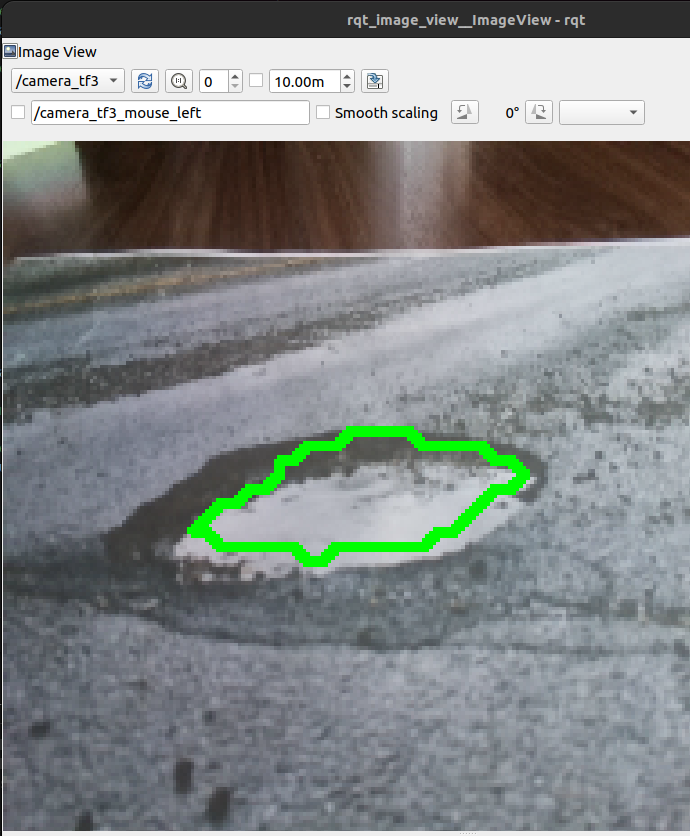
\includegraphics[width=6cm]{figs/cap6/contornobache1.png}
 %	\end{center}
 %	\caption{Versión final en la obtención del contorno del bache}
% 	\label{fig:contornobien}
% \end{figure}


\section{Modelo de cámara pinhole}
\label{sec:expmodelopinhole}

Los pasos seguidos para la aplicación del modelo pinhole para la cámara están definidos en la Sección \ref{subsec:softwarehsuelo}, pero antes de decidir si el modelo pinhole era adecuado para el proyecto, se realizaron una serie de experimentos. Para la realización de los mismos, se ha usado una cartulina de tamaño A3 pintada de cuadrados de 1x1 cm para asegurarnos que las medidas obtenidas eran lo más exactas posibles. El experimento se completa con un círculo recortado de color rosa que será detectado por un filtro de imagen y el algoritmo devolverá la posición del círculo en la vida real. Un ejemplo completo aparece en este vídeo\footnote{\url{https://www.youtube.com/watch?v=DxXaz5MFIqU}} (Figura \ref{fig:exppinhole}).

%\begin{figure} [h!]
%	\begin{center}
%			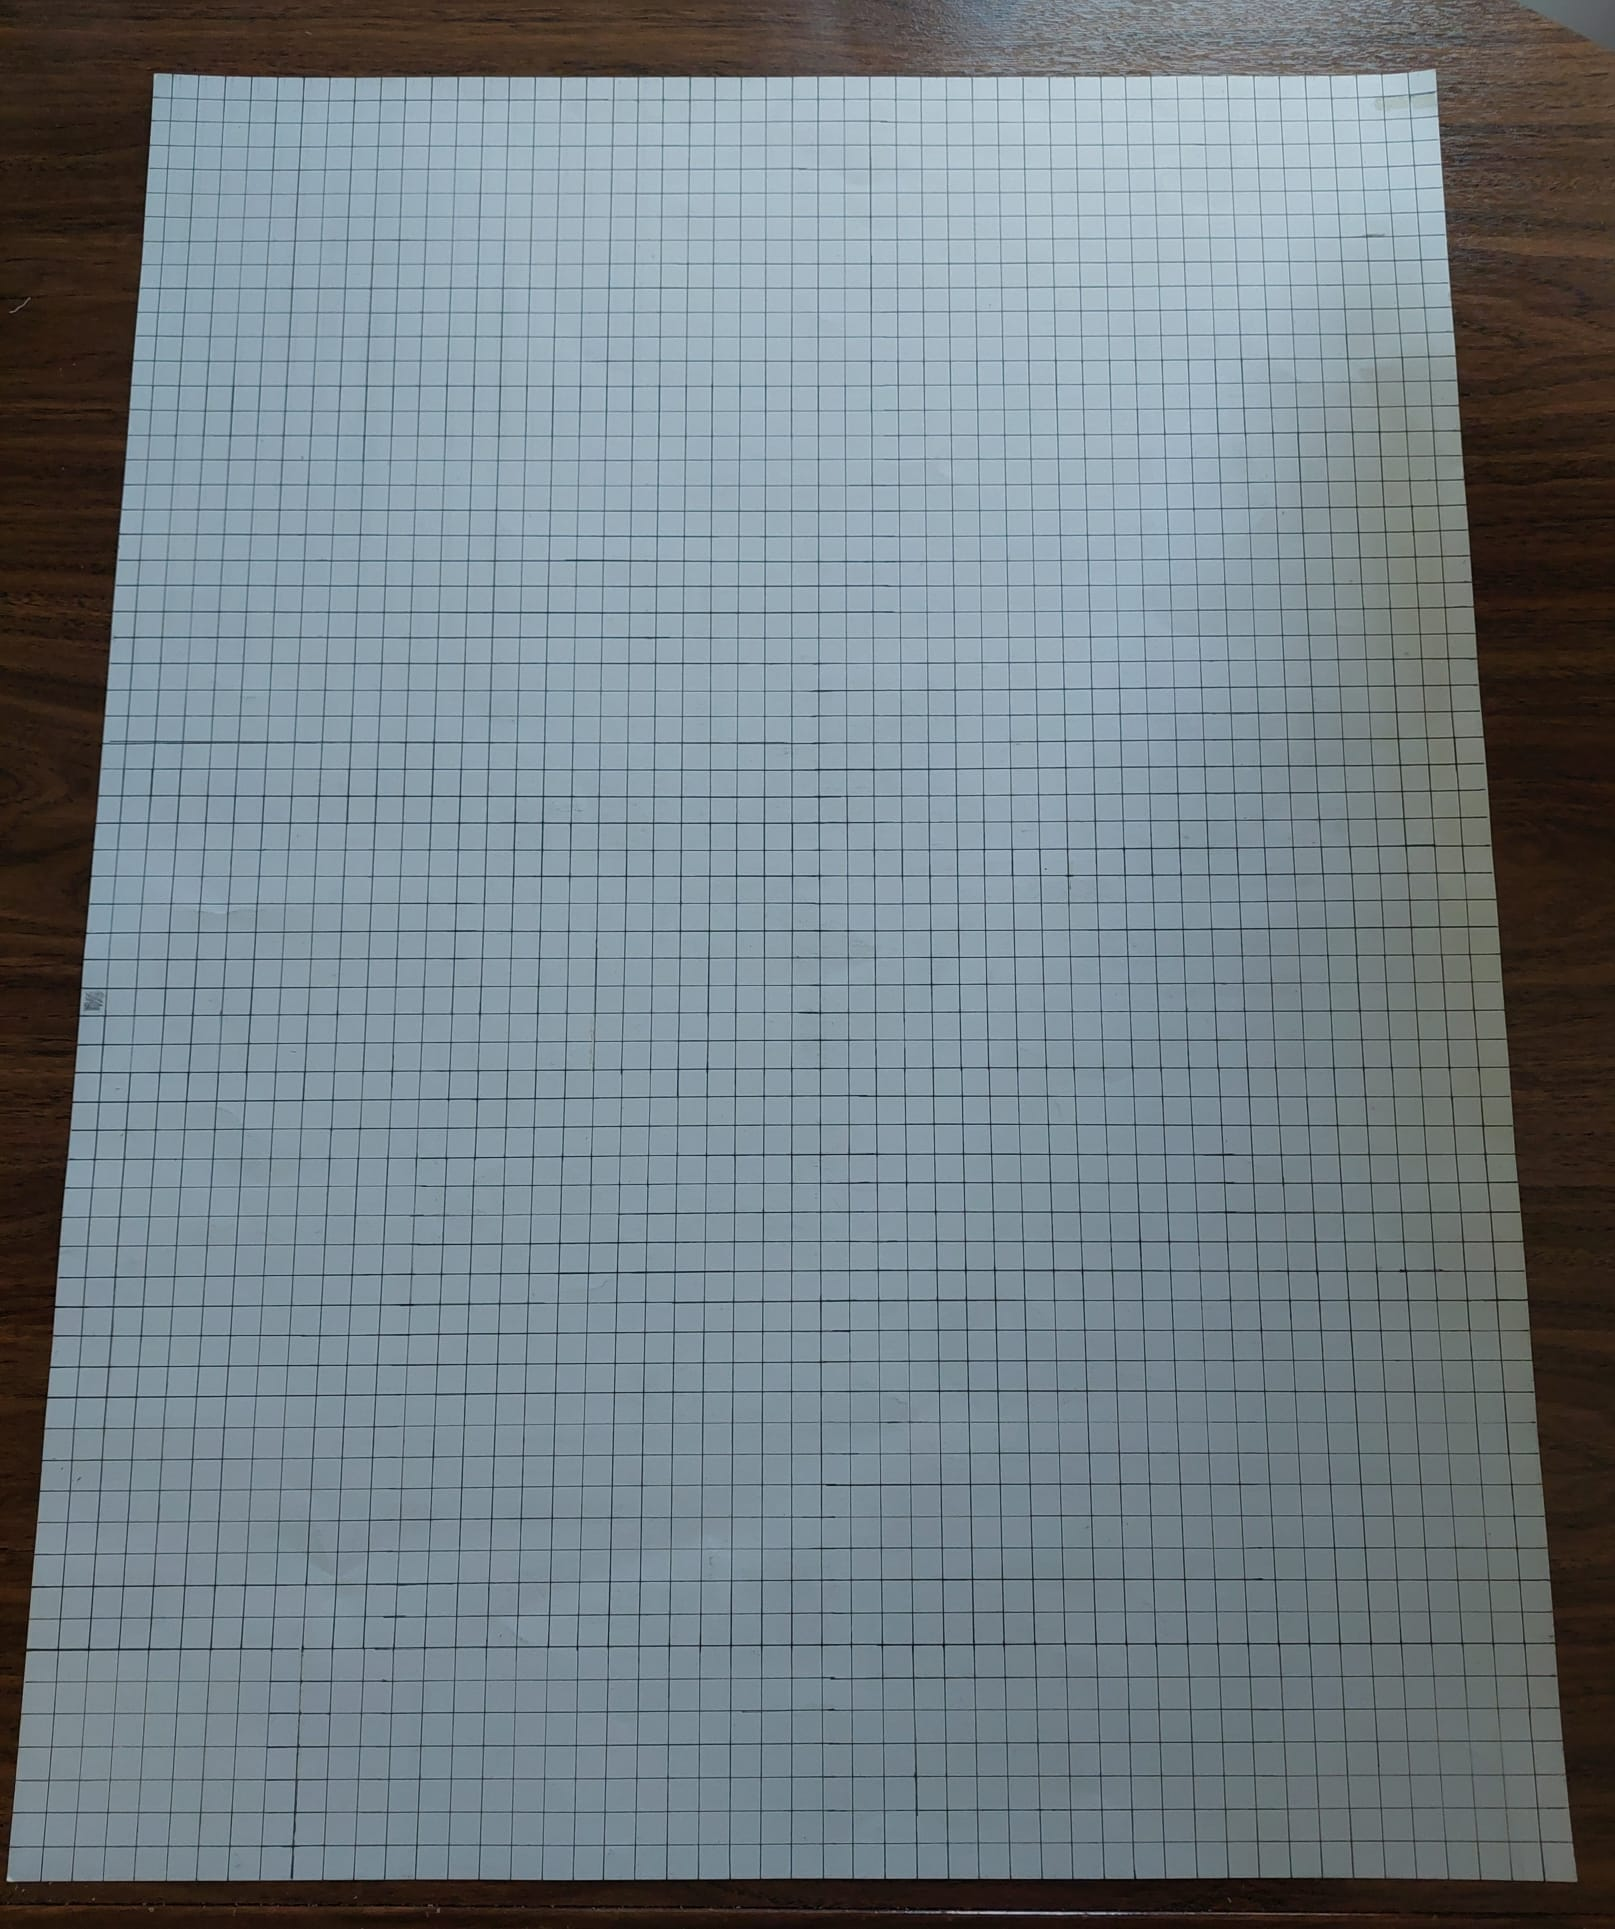
\includegraphics[width=8cm]{figs/cap7/cartulinablanca.jpeg}
%		\end{center}
%	\caption{Cartulina blanca para probar el modelo pinhole}
%	\label{fig:cartulinablanca}
%\end{figure}

%% Captura del video 

\begin{figure} [h!]
	\begin{center}
			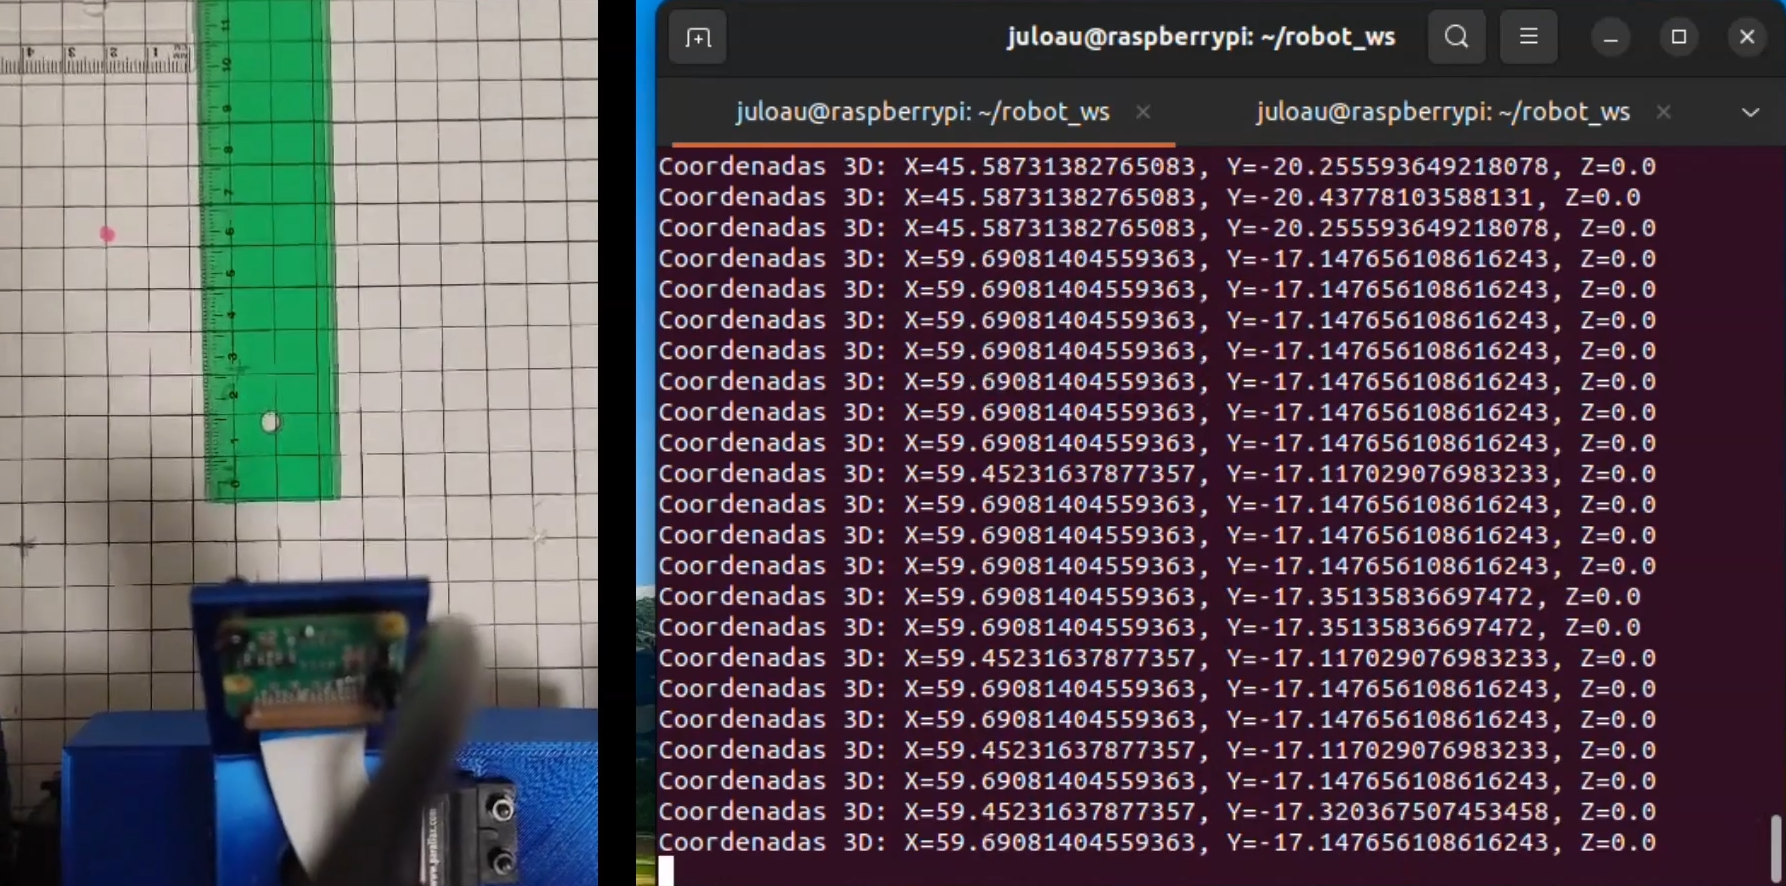
\includegraphics[width=15cm]{figs/cap7/exppinhole.png}
		\end{center}
	\caption{Captura del vídeo que demuestra el modelo pinhole}
	\label{fig:exppinhole}
\end{figure}


\section{Algoritmo de la lazada}
\label{sec:expshoelace}
Al igual que en la Sección \ref{subsec:softwareshoelace} se definió y se ejemplificó de manera teórica el funcionamiento del algoritmo de la lazada, a continuación se va a demostrar su funcionamiento pero en este caso usando un bache impreso. En la Figura \ref{fig:explazadamedidas} se puede ver las medidas reales del bache. Según la forma del bache, para demostrar que las medidas obtenidas del algoritmos son correctas, la figura que más se le parece es una elipse\footnote{\url{https://www.universoformulas.com/matematicas/geometria/area-elipse/}}. El cálculo del área teórica aparece en la Ecuación \ref{ec:areaelipse} y, por lo tanto, el área calculada usando el algoritmo de la lazada no debe superar el valor del área teórica. 

\begin{figure} [h!]
	\begin{center}
			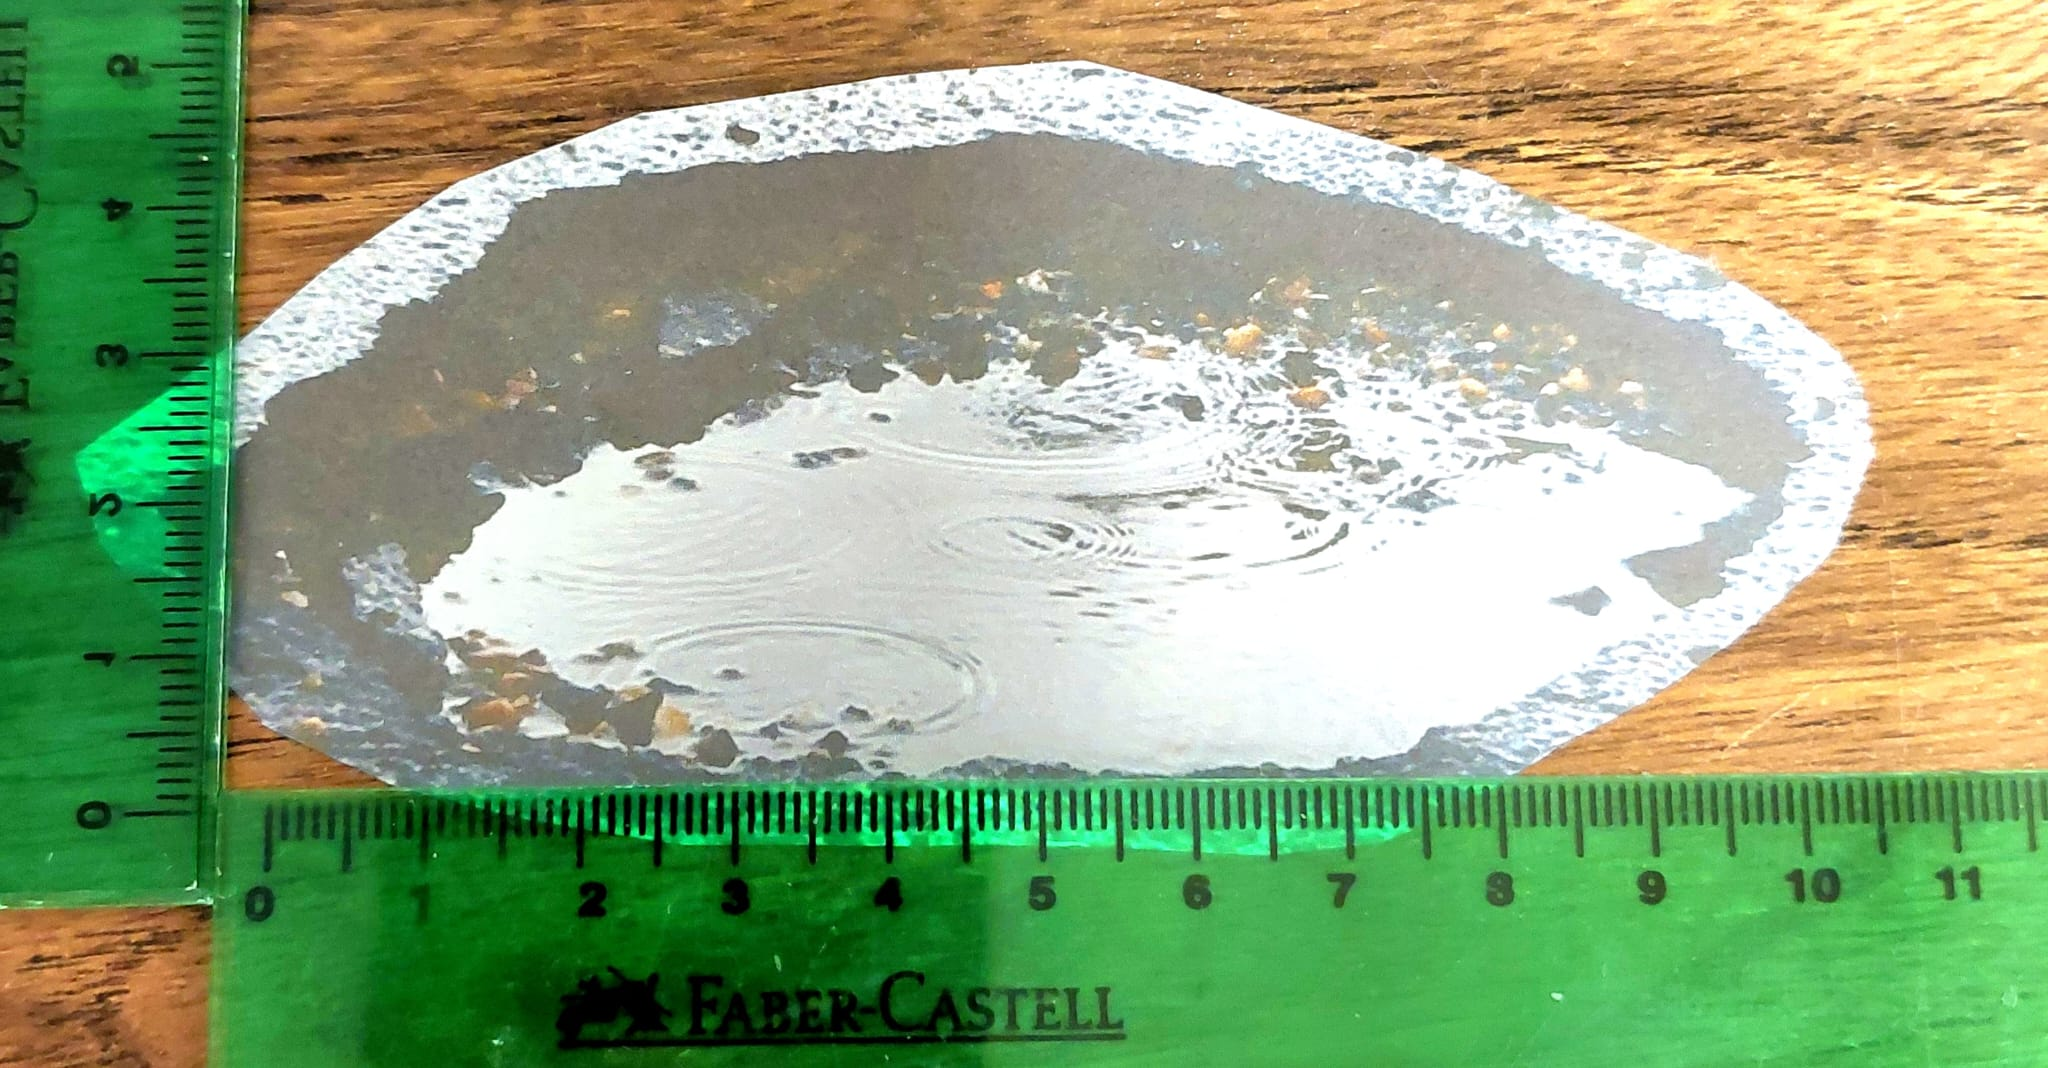
\includegraphics[width=12cm]{figs/cap7/memidasbacheteorico.jpeg}
		\end{center}
	\caption{Medidas del bache}
	\label{fig:explazadamedidas}
\end{figure}


\begin{myequation}[h]
	\begin{align}
		Area_{bache} &= R_a \cdot R_b \cdot \pi 
		\nonumber\\
		\hspace{1cm}
		Area_{bache} &= 52,2 \cdot 20 \cdot \pi = 3298,67 mm^{2}
		\nonumber
	\end{align}
	\caption[Fórmula para calcular el área de una elipse]{Fórmula para calcular el área de una elipse}
	\label{ec:areaelipse}
\end{myequation}


En el vídeo\footnote{\url{https://www.youtube.com/watch?v=E-q_aclKNqI}} (Figura \ref{fig:expcapturalazada}) se puede ver que en ningún momento el valor calculado de área no supera el valor teórico y son resultados coherentes; demostrando así que el algoritmo de la lazada es una buena opción para calcular el área.
 
%% incluir el valor del área teórica con una imagen 
%\begin{figure} [h!]
%	\begin{center}
%			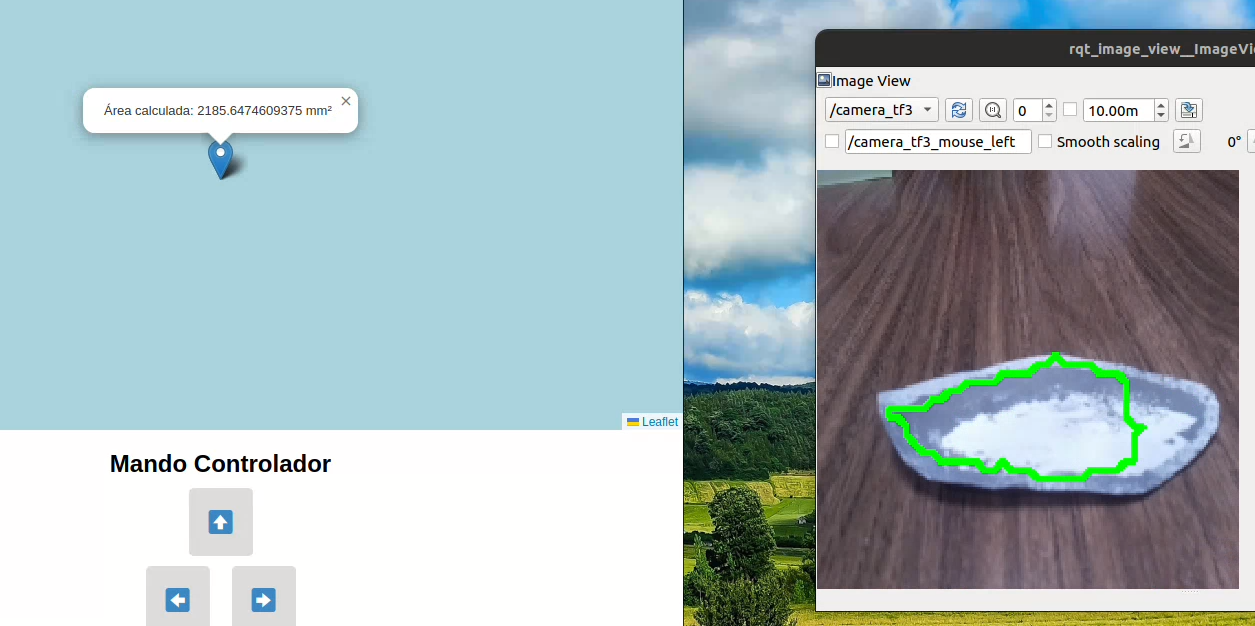
\includegraphics[width=12cm]{figs/cap7/capturavideolazada.png}
%		\end{center}
%	\caption{Captura del vídeo que calcula el área usando el algoritmo de la lazada}
%	\label{fig:expcapturalazada}
%\end{figure}

\begin{figure}[ht!]
	\centering
	\begin{minipage}{0.40\linewidth}
		\centering
		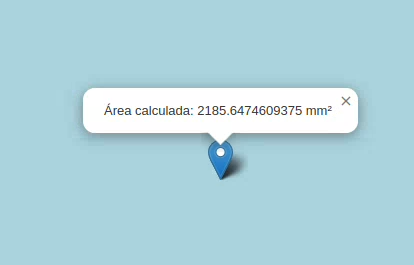
\includegraphics[width=\linewidth]{figs/cap7/capturavideolazada1.png}
	\end{minipage}
	\hspace{1cm}
	\begin{minipage}{0.40\linewidth}
		\centering
		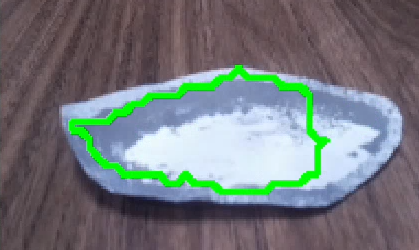
\includegraphics[width=\linewidth]{figs/cap7/capturavideolazada2.png}
	\end{minipage}
	\caption{Captura del vídeo que calcula el área usando el algoritmo de la lazada}
	\label{fig:expcapturalazada}
\end{figure}


\section{VFF}
\label{sec:expvff}
Para evitar los baches se decidió usar el algoritmo \ac{VFF}, descrito en la Sección \ref{subsec:autonomo}, y para demostrar su funcionamiento, se ha decidido crear un vídeo\footnote{\url{https://www.youtube.com/watch?v=Ka4m6CCHhxc}} que recoge los distintos casos que puede ocurrir (Figura \ref{fig:expvff}).  

 
\begin{figure} [h!]
	\centering
	\begin{minipage}{0.44\linewidth}
		\centering
		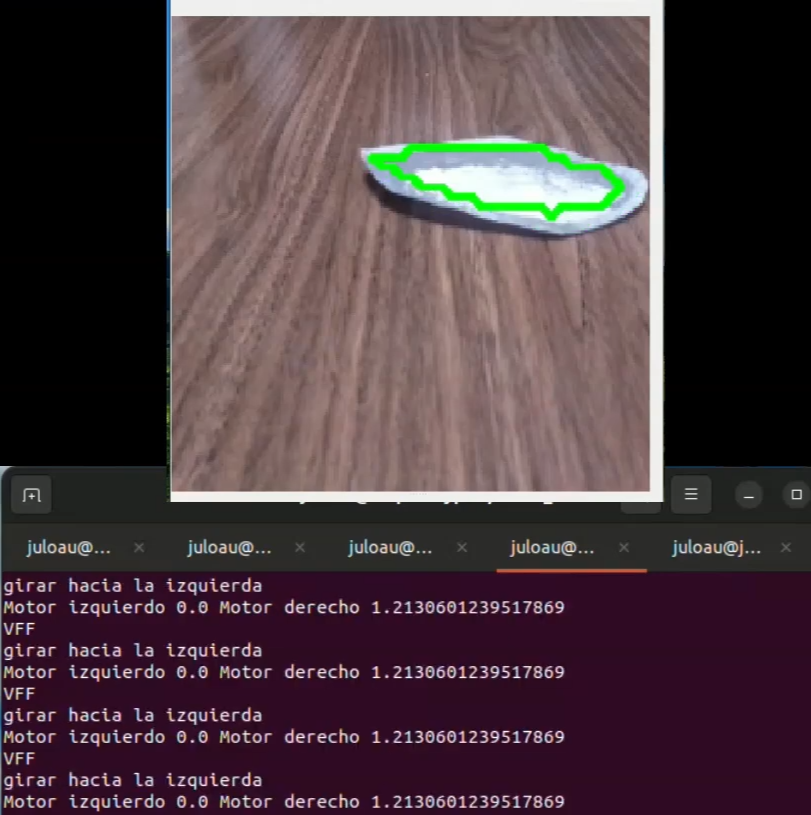
\includegraphics[width=\linewidth]{figs/cap7/demovff1.png}
	\end{minipage}
	\hspace{1cm}
	\begin{minipage}{0.45\linewidth}
		\centering
		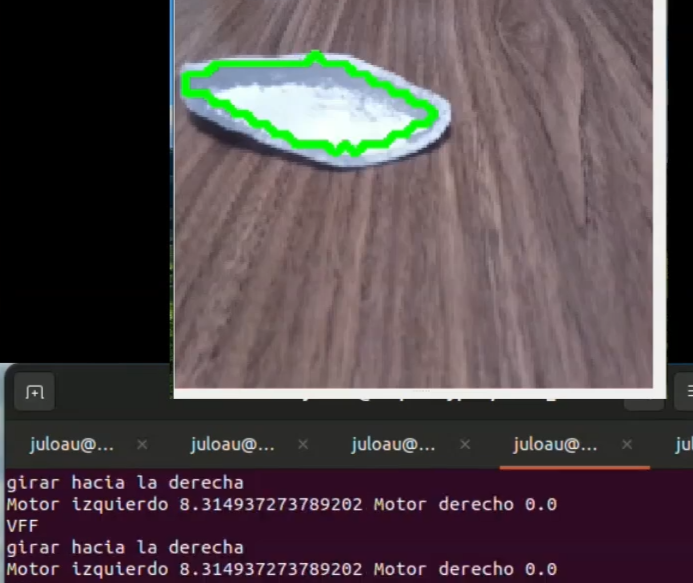
\includegraphics[width=\linewidth]{figs/cap7/demovff2.png}
	\end{minipage}
	\caption{Capturas del vídeo que hace pruebas sobre el algoritmo VFF}
	\label{fig:expvff}
\end{figure}

\section{Ejecución completa de la aplicación}
\label{sec:expcompleto}
A continuación se pueden apreciar los dos ejemplos creados que engloban las posibles opciones que existen de ejecución de PiBotJ: de forma teleoperada y de forma autónoma. Dentro de cada apartado se podrá apreciar qué comando es necesario lanzar en cada caso, un esquema de cómo funciona cada nodo dentro del \textit{launcher} y capturas de pantalla de cada vídeo. En estos ejemplos se ha calculado el volumen estimado siguiendo el valor definido por la RAC Foundation\footnote{\url{https://www.racfoundation.org/wp-content/uploads/What_is_a_pothole_final_Makwana_December_2018.pdf}}, que es de 40 mm. 

\subsection{Navegación teleoperada}

Para ejecutar PiBotJ de forma teleoperada, hay que ejecutar el \textit{launcher}: \verb|ros2 launch pibotj_rr robot_teleop.launch.py|\footnote{\url{https://github.com/RoboticsURJC/tfg-jlopez/blob/main/code/ros2/src/pibotj_rr/launch/robot_teleop.launch.py}}. Dentro del \textit{launcher} se puede distinguir una serie de nodos conectados, como muestra la Figura \ref{fig:nodosteleop}. 

\begin{figure} [h!]
	\begin{center}
			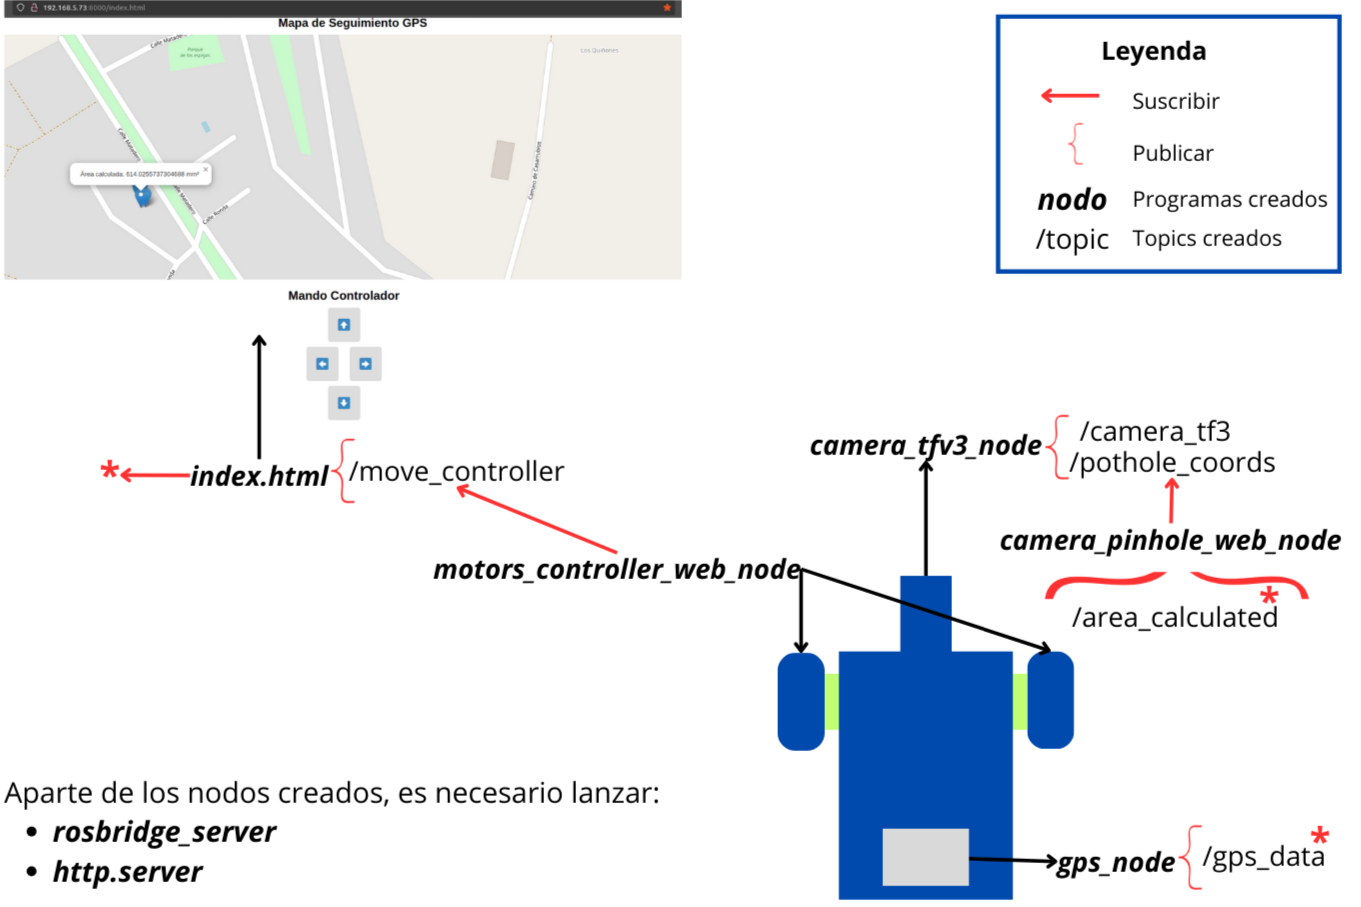
\includegraphics[width=15cm]{figs/cap7/esquema_nodos_teleop_ampliado.png}
		\end{center}
	\caption{Esquema de nodos para el modo teleoperado}
	\label{fig:nodosteleop}
\end{figure}
 
El nodo \verb|gps_node| publica la posición del robot (\verb|/gps_data|). Para poder controlar la cámara se ha creado el nodo \verb|camera_tfv3_node|, que publica la imagen de la cámara con la detección del bache (\verb|/camera_tf3|). Este se usa para la depuración, y se publican las coordenadas del contorno en el sistema de coordenadas de la imagen (\verb|/pothole_coords|). El nodo \verb|camera_pinhole_web_node| se suscribe a las coordenadas publicadas para poder convertir dichas coordenadas en el sistema de coordenadas del mundo real y poder calcular su área (\verb|/area_calculated|), la cuál será publicada. La interfaz web se suscribirá al área estimada y a los datos del \acs{GPS} para poder mostrar por pantalla el volumen estimado junto con su posición. Por otro lado, la interfaz web publica el movimiento de las ruedas (\verb|/move_controller|), a lo que el nodo \verb|motors_controller_web_node| se suscribirá a él para poder mover las ruedas según el movimiento comandado. Una ejecución completa de este ejemplo se puede apreciar en este vídeo\footnote{\url{https://www.youtube.com/watch?v=qGbJ7IGwjWk}} (Figura \ref{fig:expteleop}).
%% Capturas de pantalla del video 

\begin{figure} [h!]
	\begin{center}
		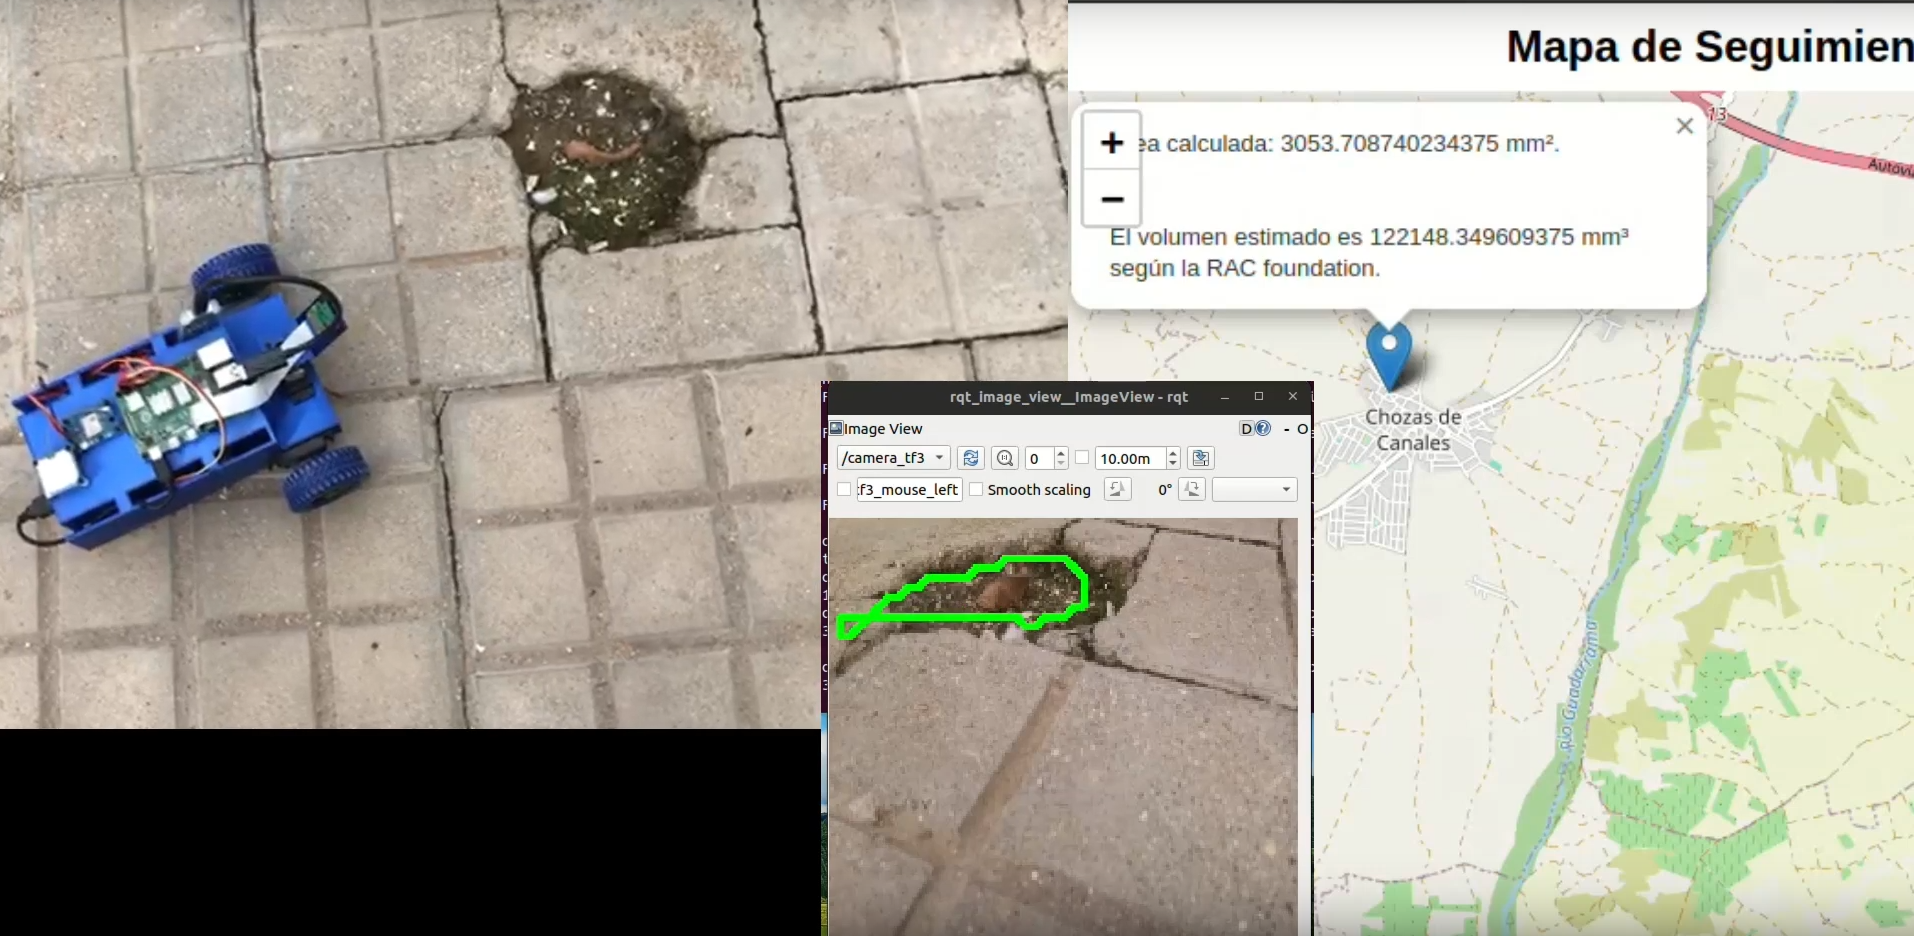
\includegraphics[width=15cm]{figs/cap7/teleop_final.png}
	\end{center}
	\caption{Captura del vídeo del modo teleoperado}
	\label{fig:expteleop}
\end{figure}


\subsection{Navegación autónoma}

Para ejecutar PiBotJ de forma autónoma hay que ejecutar el \textit{launcher}: \verb|ros2 launch pibotj_rr robot_vff.launch.py|\footnote{\url{https://github.com/RoboticsURJC/tfg-jlopez/blob/main/code/ros2/src/pibotj_rr/launch/robot_vff.launch.py}}. Dentro del \textit{launcher} se puede distinguir una serie de nodos conectados, como muestra la Figura \ref{fig:nodosvff}. 


\begin{figure} [h!]
	\begin{center}
			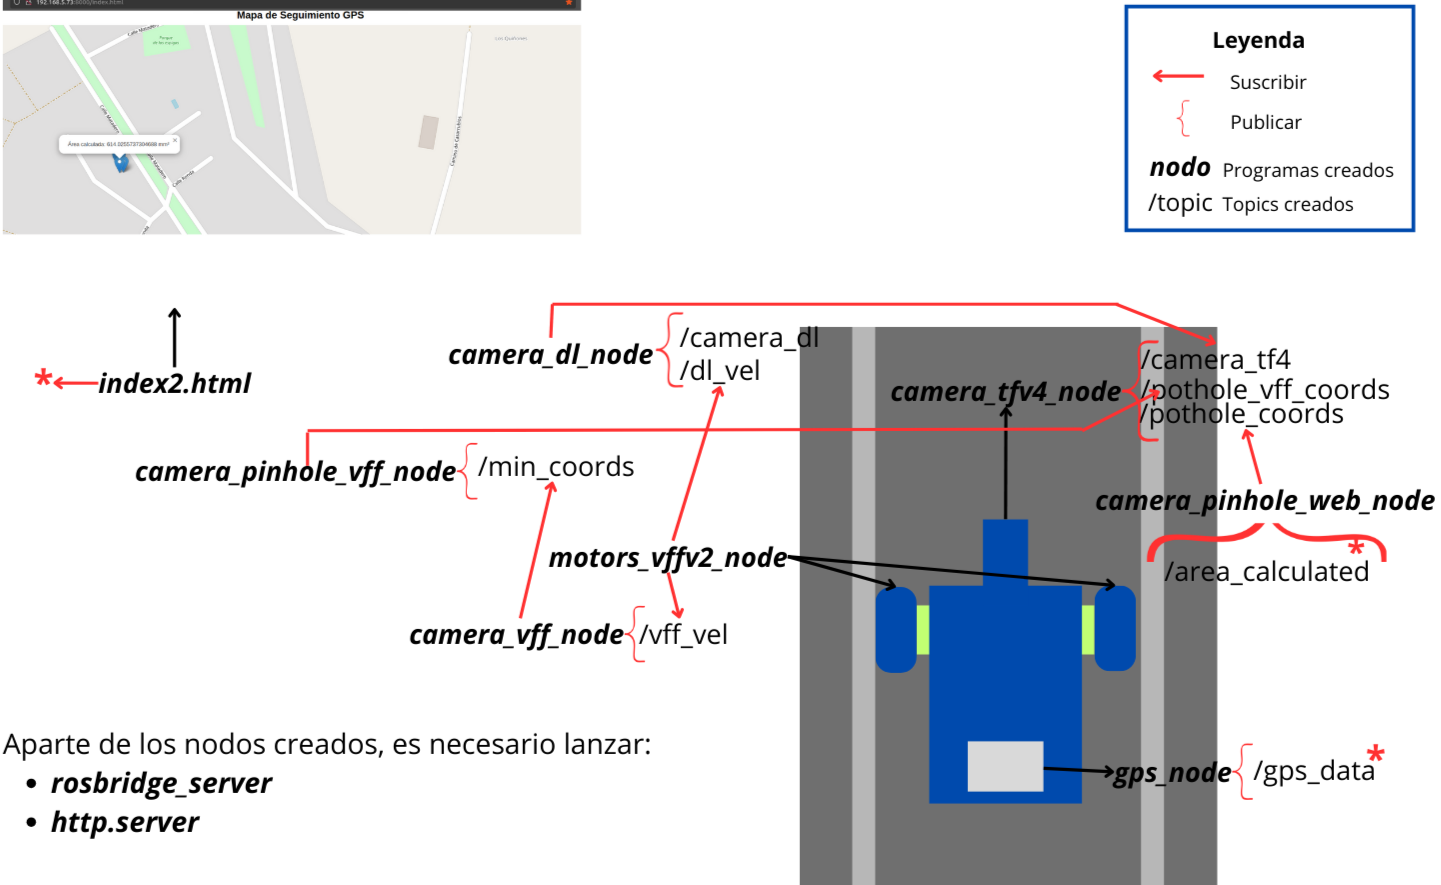
\includegraphics[width=15cm]{figs/cap7/esquema_nodos_vff_ampliado.png}
		\end{center}
	\caption{Esquema de nodos para el modo autónomo}
	\label{fig:nodosvff}
\end{figure}


El nodo \verb|gps_node| publica la posición del robot (\verb|/gps_data|). Para controlar la cámara se ha creado el nodo \verb|camera_tfv4_node|, que publica la imagen de la cámara con la detección del bache (\verb|/camera_tf4|), y se publican dos veces las coordenadas del contorno en el sistema de coordenadas de la imagen (\verb|/pothole_coords| y \verb|/pothole_vff_coords|). La diferencia que existe entre cada \textit{topic} es que el primero se publica cada dos segundos y el segundo cada segundo. El nodo \verb|camera_pinhole_web_node| se suscribe a las coordenadas publicadas (\verb|/pothole_coords|) para poder convertir dichas coordenadas en el sistema de coordenadas del mundo real y, de este modo, poder calcular su área (\verb|/area_calculated|), la cuál será publicada. La interfaz web se suscribirá al área calculado y a los datos del \acs{GPS} para poder mostrar por pantalla el volumen estimado junto con su posición. 

Por otro lado, el nodo \verb|camera_pinhole_vff_node| se suscribe a las coordenadas publicadas (\verb|/pothole_vff_node|) para convertirlas en el sistema de coordenadas del mundo real hasta encontrar la coordenada que se encuentra más cerca del robot (usando el eje X) para posteriormente ser publicada (\verb|/min_coords|). Es el nodo \verb|camera_vff_node| quien se suscribe a la coordenada menor para poder aplicar el algoritmo \acs{VFF} y que, de este modo, se pueda—finalmente—publicar una velocidad resultante (\verb|/vff_vel|).

Para completar el comportamiento final el nodo \verb|camera_dl_node| se suscribe a la imagen con la detección del bache para poder aplicar un filtro de detección de líneas. Se publica la imagen con el filtro aplicado (\verb|/camera_dl|), usado para depuración, y una velocidad resultante (\verb|/dl_vel|), dependiendo de la situación.

Finalmente, es el nodo \verb|motors_vffv2_node| quien se suscribirá a las dos velocidades y dará prioridad a la detección de baches antes que a la detección de líneas, para aplicar la velocidad adecuada a los motores, usando mecanismos de sincronización.

Una ejecución completa de este ejemplo se puede apreciar en este vídeo\footnote{\url{https://www.youtube.com/watch?v=zQudXBXHVaY}} (Figura \ref{fig:expvfffinal}). 

\begin{figure} [h!]
	\begin{center}
		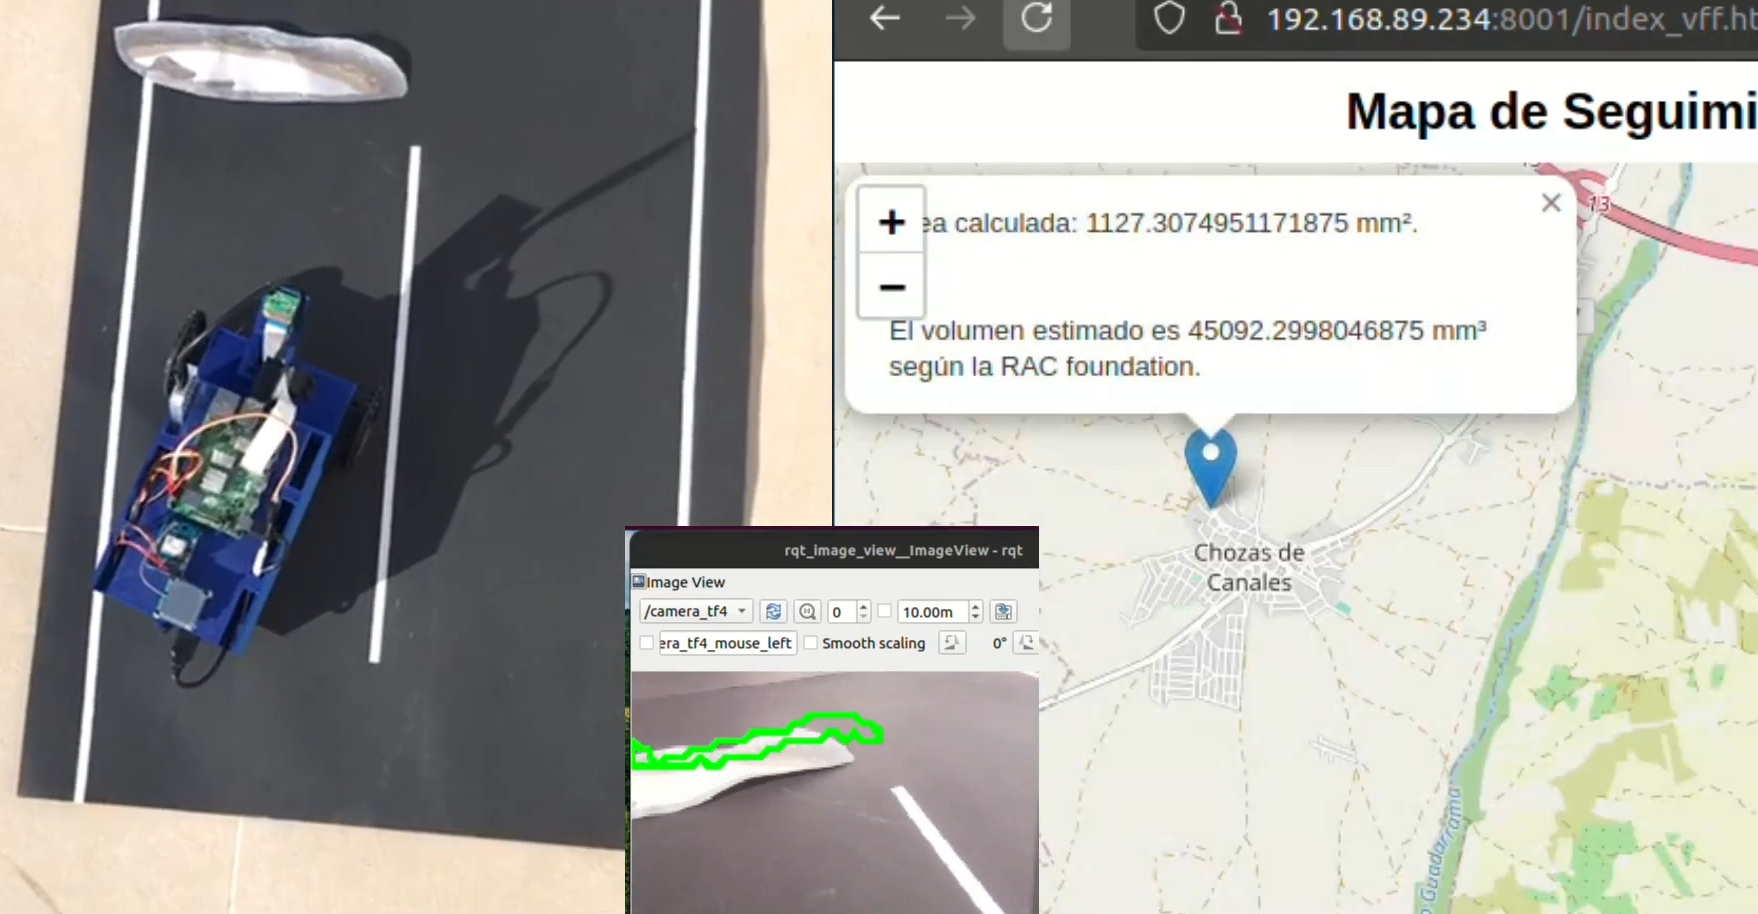
\includegraphics[width=15cm]{figs/cap7/autonomo_final.png}
	\end{center}
	\caption{Captura del vídeo del modo autónomo}
	\label{fig:expvfffinal}
\end{figure}

